\begin{figure}[H]
\centering
\caption{Share of couples by women's relative income by year}
\label{fig:figure_3}
\subfloat[1990]{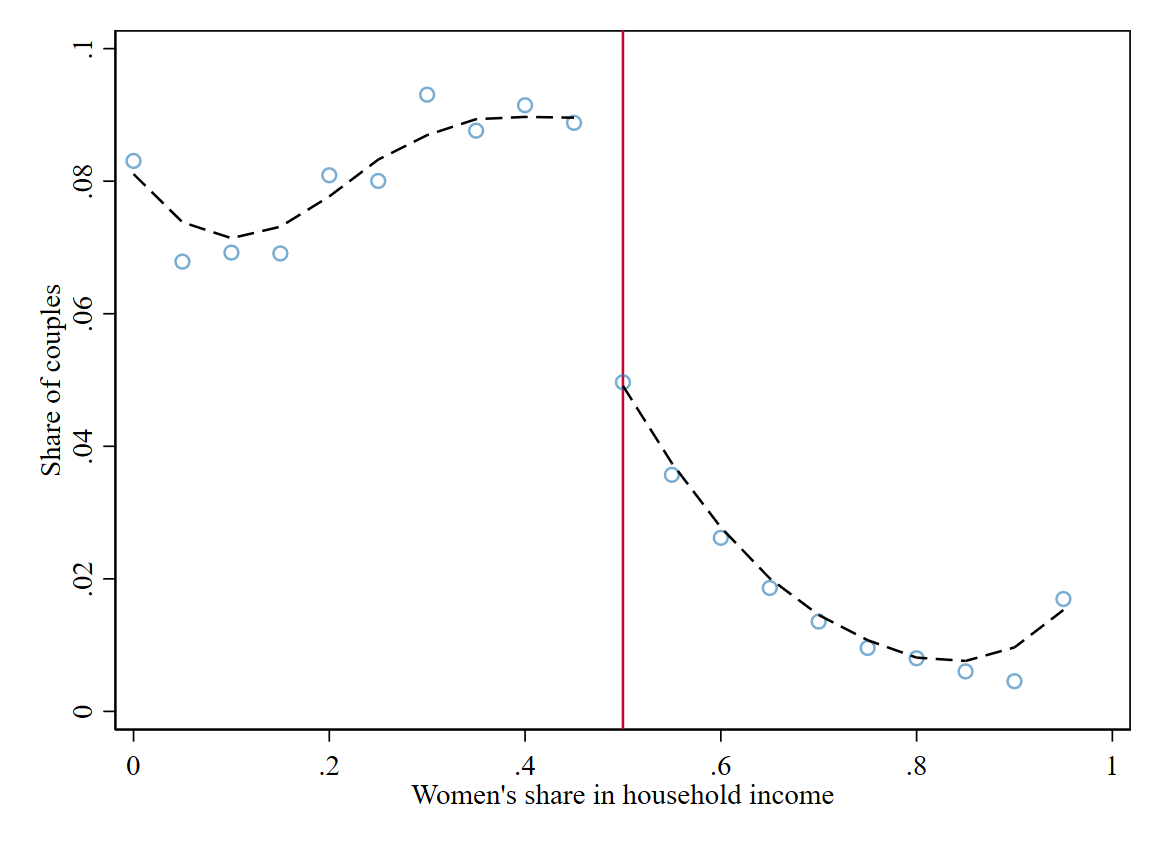
\includegraphics[width=.5\textwidth]{../../results/figures/figure_3_1990.png}} \subfloat[2000]{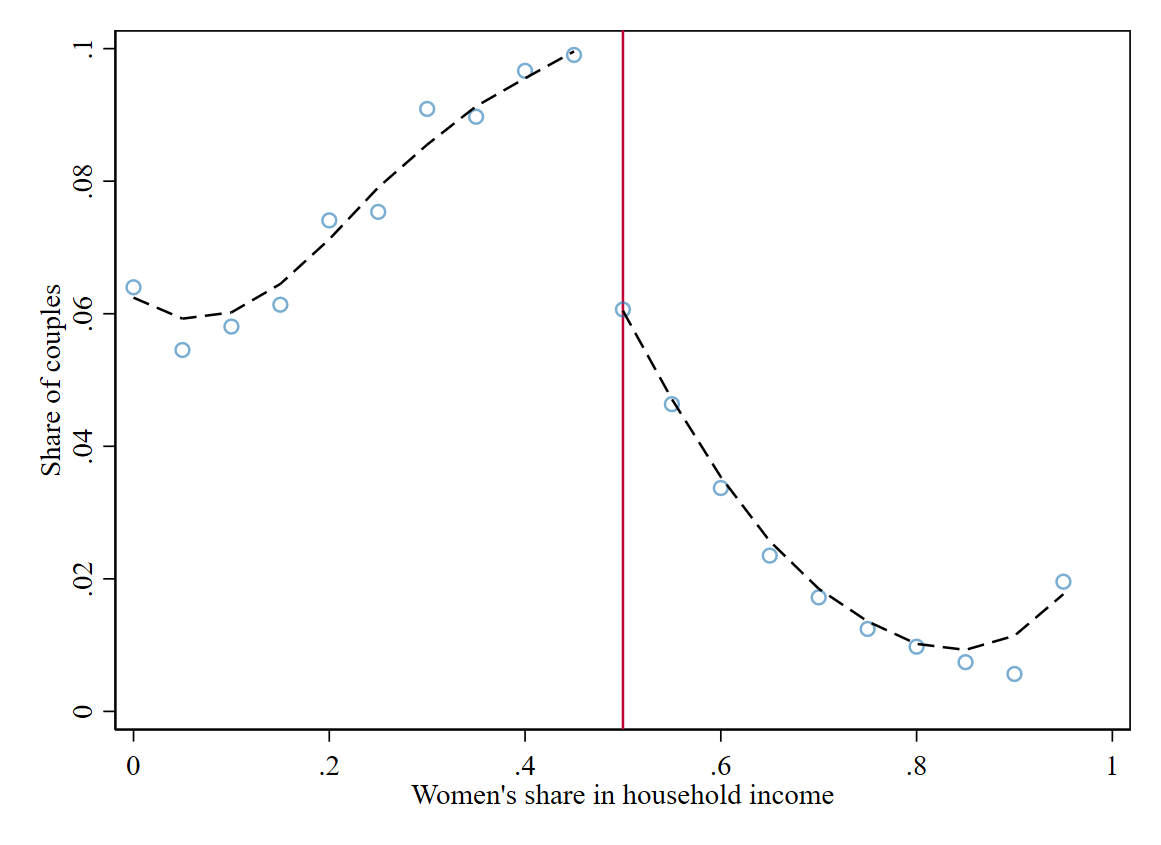
\includegraphics[width=.5\textwidth]{../../results/figures/figure_3_2000.png}} \\ \subfloat[2011]{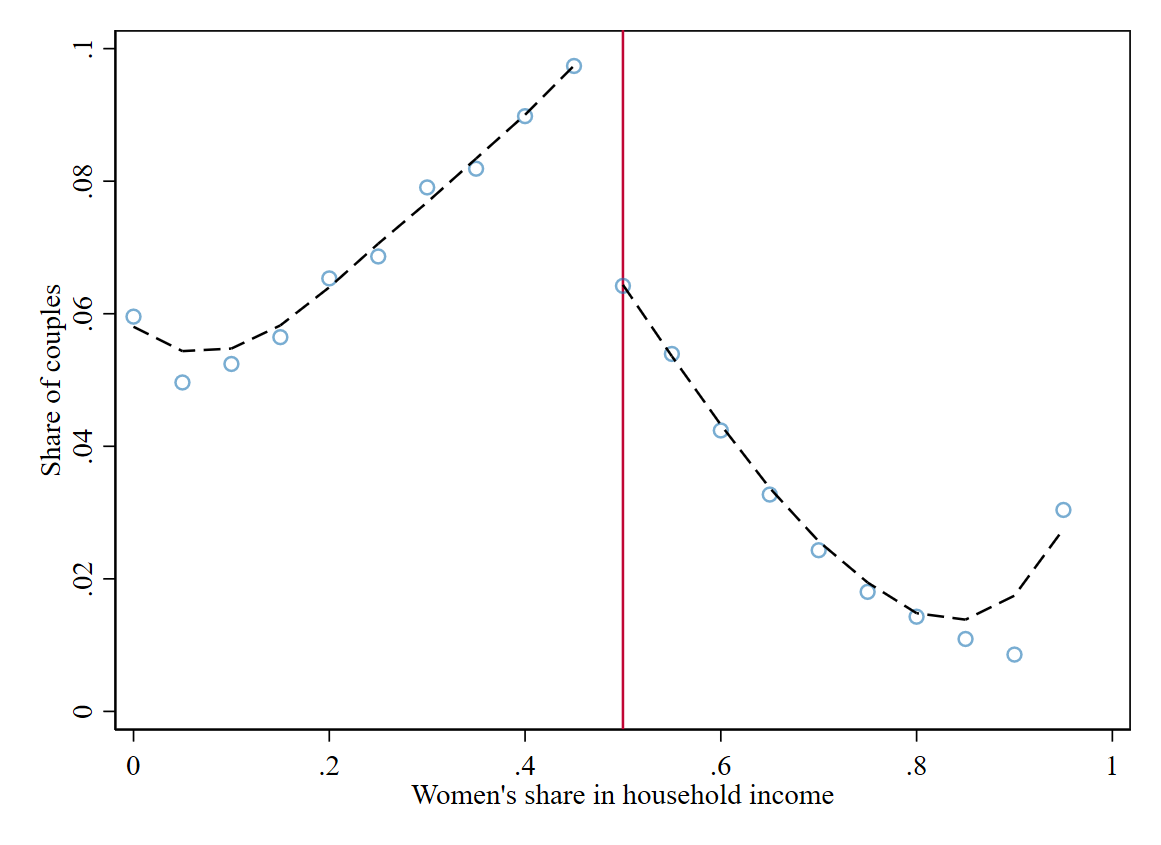
\includegraphics[width=.5\textwidth]{../../results/figures/figure_3_2011.png}} 
\par \begin{minipage}[h]{\textwidth}{\scriptsize\textit{Notes:} Each dot represents a bin of size 0.05 of the relative income share. Vertical line marks couples where the woman earns 50\% of the couples income.}\end{minipage}
\end{figure}
